% ============================================================
%  TEMPLATE PENULISAN ILMIAH
%  Program Studi Informatika – Universitas Gunadarma
%  Berdasarkan Buku Pedoman Penulisan Ilmiah 2025
% ============================================================
\documentclass[12pt, a4paper]{report}

% ----- Package -----
\usepackage[T1]{fontenc}
\usepackage[utf8]{inputenc}
\usepackage{mathptmx}           % Times New Roman
\usepackage[bahasa]{babel}
\usepackage{natbib}
\usepackage{geometry}
\usepackage{setspace}
\usepackage{titlesec}
\usepackage{titletoc}
\usepackage{tocloft}
\usepackage{fancyhdr}
\usepackage{graphicx}
\usepackage{float}
\usepackage{caption}
\usepackage{tabularx}
\usepackage{booktabs}
\usepackage{indentfirst}
\usepackage{parskip}
\usepackage{microtype}
\usepackage{afterpage}
\usepackage{emptypage}          % halaman kosong tidak ada header/footer
\usepackage{etoolbox}
\usepackage[hidelinks, plainpages=false, hypertexnames=false]{hyperref}
\usepackage{bookmark}
\usepackage{color}





% ----- Geometry (Margin) -----
% Atas: 4cm | Bawah: 3cm | Kiri: 4cm | Kanan: 3cm
\geometry{
  a4paper,
  top    = 4cm,
  bottom = 3cm,
  left   = 4cm,
  right  = 3cm
}

% ----- Spasi 1.5 (isi utama) -----
\setstretch{1.5}

% ============================================================
%  DATA MAHASISWA – ubah bagian ini saja
% ============================================================
\newcommand{\NamaMahasiswa}{Anaf Naufalian}
\newcommand{\NPM}{50423155}
\newcommand{\JudulPI}{Dalsilens: A Real-Time Mobile Assistive Tool for Dichromacy Using LMS Daltonization and HSV-Based Color Identification}
\newcommand{\JudulPISatu}{Dalsilens: A Real-Time Mobile Assistive Tool for Dichromacy Using LMS Daltonization and HSV-Based Color Identification} % tanpa newline, untuk header dll
\newcommand{\NamaPembimbing}{Dr. Bonang Waspadadi Ligar, S.Si., M.MSi.}
\newcommand{\TanggalSidang}{01 Januari 2026}
\newcommand{\TanggalLulus}{01 Januari 2026}
\newcommand{\TanggalACC}{01 Januari 2026}
\newcommand{\BulanTahun}{Januari 2026}
\newcommand{\Tahun}{2026}
\newcommand{\KataKunci}{katakunci1, katakunci2, katakunci3}
\newcommand{\Keywords}{Color Vision Deficiency, Dichromacy, Daltonization, LMS Color Space, Real-Time Image Processing, Android}

% ============================================================
%  FORMAT JUDUL BAB & SUBBAB
%  Bab  : 14pt, Bold, Kapital, Tengah
%  Sub  : 12pt, Bold, Kapital awal kata, Kiri
% ============================================================

% -- Judul Bab (BAGIAN) --
\titleformat{\chapter}[block]
  {\centering\bfseries\fontsize{14}{16}\selectfont}
  {\thechapter.}
  {0.5em}
  {\MakeUppercase}
\titlespacing*{\chapter}{0pt}{0pt}{3\baselineskip}

% -- Subbab --
\titleformat{\section}[block]
  {\bfseries\fontsize{12}{14}\selectfont}
  {\thesection.}
  {0.5em}
  {}
\titlespacing*{\section}{0pt}{2\baselineskip}{1\baselineskip}

% -- Sub-subbab --
\titleformat{\subsection}[block]
  {\bfseries\fontsize{12}{14}\selectfont}
  {\thesubsection.}
  {0.5em}
  {}
\titlespacing*{\subsection}{0pt}{2\baselineskip}{1\baselineskip}

% Gunakan angka Arab (1, 2, 3 …) bukan Roman
\renewcommand{\thechapter}{\arabic{chapter}}
\renewcommand{\thesection}{\thechapter.\arabic{section}}
\renewcommand{\thesubsection}{\thesection.\arabic{subsection}}

% ============================================================
%  CAPTION GAMBAR & TABEL
%  Gambar : bawah tengah
%  Tabel  : atas tengah
% ============================================================
\captionsetup[figure]{
  labelfont=bf,
  font=normalsize,
  justification=centering,
  position=below
}
\captionsetup[table]{
  labelfont=bf,
  font=normalsize,
  justification=centering,
  position=above
}
% Penomoran: Gambar 1.1, Tabel 2.3, dst.
\renewcommand{\thefigure}{\thechapter.\arabic{figure}}
\renewcommand{\thetable}{\thechapter.\arabic{table}}

% ============================================================
%  HEADER & FOOTER
% ============================================================
\pagestyle{fancy}
\fancyhf{}
% Halaman biasa (bukan awal bab): nomor di pojok kanan atas
\fancyhead[R]{\thepage}
\renewcommand{\headrulewidth}{0pt}

% Awal bab: nomor di tengah bawah
\fancypagestyle{chapterpage}{
  \fancyhf{}
  \fancyfoot[C]{\thepage}
  \renewcommand{\headrulewidth}{0pt}
}
\AtBeginEnvironment{document}{}

% ============================================================
%  DAFTAR ISI / TABEL / GAMBAR – format TNR 12, single
% ============================================================
\renewcommand{\cfttoctitlefont}{\hfill\bfseries\fontsize{12}{14}\selectfont\MakeUppercase}
\renewcommand{\cftaftertoctitle}{\hfill}
\renewcommand{\cftlottitlefont}{\hfill\bfseries\fontsize{12}{14}\selectfont\MakeUppercase}
\renewcommand{\cftafterlottitle}{\hfill}
\renewcommand{\cftloftitlefont}{\hfill\bfseries\fontsize{12}{14}\selectfont\MakeUppercase}
\renewcommand{\cftafterloftitle}{\hfill}

\setlength{\cftbeforetoctitleskip}{0pt}
\setlength{\cftaftertoctitleskip}{3\baselineskip}
\setlength{\cftbeforechapskip}{0pt}

% Bab di daftar isi: Bold, Kapital
\renewcommand{\cftchapfont}{\bfseries}
\renewcommand{\cftchappagefont}{\bfseries}
\renewcommand{\cftchapleader}{\cftdotfill{\cftdotsep}}

% ============================================================
%  HYPERREF (nonaktifkan warna link untuk cetak)
% ============================================================
\hypersetup{
  colorlinks    = false,
  hidelinks,
  plainpages    = false,
  hypertexnames = false,
  bookmarksopen = true,       % <-- sidebar langsung terbuka
  bookmarksnumbered = true,   % <-- tampilkan nomor bab
}


% ============================================================
%  MULAI DOKUMEN
% ============================================================
\begin{document}

% ============================================================
%  BAGIAN AWAL – penomoran romawi kecil
% ============================================================
\pagenumbering{roman}
\setcounter{page}{1}
% ============================================================
%  HALAMAN JUDUL
%  Pedoman: semua center, TNR, logo 6cm, judul 14pt bold kapital
%  Catatan: halaman ini dihitung (i) tapi nomor tidak dicetak
% ============================================================

\phantomsection
\thispagestyle{empty}

\begin{center}
\singlespacing

{\fontsize{14}{14}\selectfont\bfseries UNIVERSITAS GUNADARMA\\
\fontsize{12}{14}\selectfont FAKULTAS TEKNOLOGI INDUSTRI}

\vspace{1.5cm}

% Logo Gunadarma – ganti dengan file logo asli (diameter 6cm = ~170px)
% Letakkan file logo di folder gambar/

\includegraphics[width=6cm]{gambar/logo-gundar}

\vspace{1.5cm}

{\fontsize{14}{16}\selectfont\bfseries
PENULISAN ILMIAH\\[0.5em]
\MakeUppercase{\JudulPI}
}

\vspace{2.5cm}

\begin{tabular}{l@{\hspace{0.5cm}:\hspace{0.5cm}}l}
  \textbf{Nama}            & \NamaMahasiswa \\
  \textbf{NPM}             & \NPM \\
  \textbf{Program Studi}   & Informatika \\
  \textbf{Pembimbing}      & \NamaPembimbing \\
\end{tabular}

\vfill

{\fontsize{12}{14}\selectfont\bfseries
JAKARTA\\[0.3em]
\Tahun
}

\end{center}

\newpage
       % di dalam: \thispagestyle{empty} saja, tanpa addcontentsline
% ============================================================
%  HALAMAN PERNYATAAN ORISINALITAS DAN PUBLIKASI
%  Pedoman: TNR 12pt, spasi 1.5, justify
% ============================================================
\thispagestyle{chapterpage}
\phantomsection
\addcontentsline{toc}{chapter}{PERNYATAAN ORISINALITAS DAN PUBLIKASI}
\pagestyle{chapterpage}

\begin{center}
  {\bfseries\fontsize{12}{14}\selectfont
  PERNYATAAN ORISINALITAS DAN PUBLIKASI}
\end{center}

\vspace{2\baselineskip}

Saya yang bertanda tangan di bawah ini,

\vspace{1\baselineskip}

\noindent
\begin{tabular}{p{3.5cm} c p{9cm}}
  Nama            & : & \NamaMahasiswa \\[0.5em]
  NPM             & : & \NPM \\[0.5em]
  Judul PI        & : & \JudulPISatu \\[0.5em]
  Tanggal Sidang  & : & \TanggalSidang \\[0.5em]
  Tanggal Lulus   & : & \TanggalLulus \\
\end{tabular}

\vspace{1\baselineskip}

\noindent
menyatakan bahwa tulisan ini adalah merupakan hasil karya saya sendiri dan dapat
dipublikasikan sepenuhnya oleh Universitas Gunadarma. Segala kutipan dalam bentuk
apa pun telah mengikuti kaidah, etika yang berlaku. Mengenai isi dan tulisan adalah
merupakan tanggung jawab Penulis, bukan Universitas Gunadarma. Demikian pernyataan
ini dibuat dengan sebenarnya dan dengan penuh kesadaran.

\vspace{1\baselineskip}

\noindent
\begin{minipage}[t]{0.35\textwidth}
  \raisebox{-\height}{% <-- turunkan fbox agar baseline-nya di atas
    \fbox{\begin{minipage}[c][4.2cm][c]{3.2cm}
            \centering
            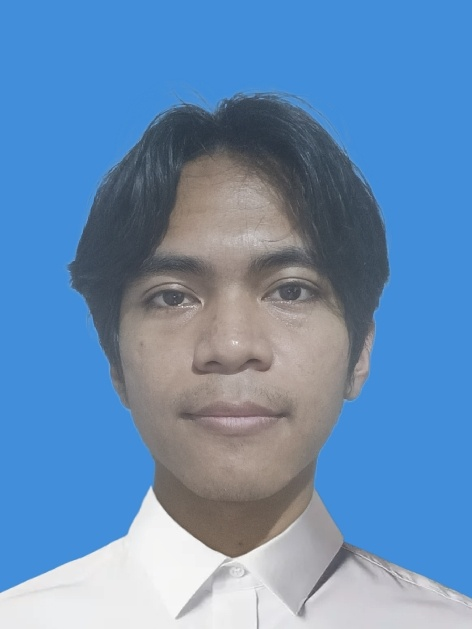
\includegraphics[width=3cm,height=4cm,keepaspectratio]{gambar/passphoto}
    \end{minipage}}%
  }
\end{minipage}
\hfill
\begin{minipage}[t]{0.55\textwidth}
  \vspace{0.02cm}
  Jakarta, \TanggalACC

  \vspace{0.5cm}


  
\includegraphics[width=3cm]{gambar/signature}\\[-0.3em]
  (\NamaMahasiswa)
\end{minipage}

\newpage
\pagestyle{chapterpage}
 % di dalam: \phantomsection lalu \addcontentsline lalu konten
% ============================================================
%  HALAMAN PENGESAHAN
%  Pedoman: TNR 12pt, spasi 1
% ============================================================

\phantomsection
\thispagestyle{empty}
\addcontentsline{toc}{chapter}{LEMBAR PENGESAHAN}
\pagestyle{chapterpage}

{\singlespacing

\begin{center}
  {\bfseries\fontsize{14}{14}\selectfont LEMBAR PENGESAHAN}
\end{center}

\vspace{2\baselineskip}

\noindent
\begin{tabular}{p{3.5cm} c p{9cm}}
  Judul PI        & : & \JudulPISatu \\[0.5em]
  Nama            & : & \NamaMahasiswa \\[0.5em]
  NPM             & : & \NPM \\[0.5em]
  Program Studi   & : & Informatika \\[0.5em]
  Tanggal Sidang  & : & \TanggalSidang \\[0.5em]
  Tanggal Lulus   & : & \TanggalLulus \\
\end{tabular}

\vspace{3\baselineskip}

\begin{center}
  Menyetujui
\end{center}

\vspace{2\baselineskip}

\noindent
\begin{minipage}[t]{0.45\textwidth}
  \centering
  Pembimbing

  \vspace{2.5cm}

  (\NamaPembimbing)
%  \mbox{(\NamaPembimbing)}
\end{minipage}
\hfill
\begin{minipage}[t]{0.45\textwidth}
  \centering
  Kasubbag. Sidang PI

  \vspace{2.5cm}

%  \mbox{( Dr. Achmad Fahrurozi, S.Si., M.Si. )}
  (Dr. Achmad Fahrurozi, S.Si., M.Si.)
\end{minipage}

\vspace{3\baselineskip}

\begin{center}
  Ketua Program Studi

  \vspace{2.5cm}

  (Prof. Dr. Lintang Yuniar Banowosari, S.Kom., M.Sc.)
\end{center}

} % end singlespacing

\newpage
\pagestyle{chapterpage}
% ============================================================
%  ABSTRAK (Bahasa Indonesia & Inggris)
%  Pedoman: TNR 12pt, single spacing, maks 200 kata per bahasa
% ============================================================

\phantomsection
\thispagestyle{chapterpage}
\addcontentsline{toc}{chapter}{ABSTRAK}

{\singlespacing

%% ---- Abstrak Bahasa Indonesia ----
%\begin{center}
%  {\bfseries ABSTRAK}
%\end{center}
%
%\noindent
%\NamaMahasiswa, \NPM \\
%\MakeUppercase{\JudulPISatu}\\
%Penulisan Ilmiah. Informatika. Fakultas Teknologi Industri. Universitas Gunadarma. \Tahun
%
%\noindent
%Kata Kunci: \KataKunci\\
%(xii + 62 + Lampiran)
%
%\medskip
%\noindent
%% Isi abstrak – maksimum 200 kata, 1 paragraf
%Color Vision Deficiency (CVD), commonly known as color blindness,is a genetic condition that affects a person's capacity ability to differentiate between certain light wavelengths.
%Although eyesight itself is usually normal, individuals with CVD find it difficult to distinguish colors within the red, green, and blue spectrums.
%The most common type is Dichromacy, which includes Protanopia (red-blind), Deuteranopia (green-blind), and Tritanopia (blue-blind).
%Existing assistive technologies, such as color-filtering glasses, are designed to separate overlapping red and green wavelengths, help with color distinction but are often expensive.
%Additionally, many existing smartphone applications require users to upload images for processing, which prevents real-time operation and limits immediate visual feedback.
%This paper proposes the implementation of the LMS Daltonization algorithm on the Android platform using real-time image processing.
%The method converts the camera's input from the RGB color space to the LMS color space.
%This allows for the mathematical simulation and adjustment of the missing color spectrums.
%The application is expected to help users distinguish objects with specific color spectrum through a smartphone, with low latency that supports real-time usage.
%
%\noindent
%Daftar Pustaka (<<tahun awal>> -- <<tahun akhir>>)
%
%\vspace{2\baselineskip}

% ---- Abstract Bahasa Inggris ----
\begin{center}
  {\bfseries ABSTRACT}
\end{center}

\noindent
\NamaMahasiswa, \NPM \\
\MakeUppercase{\JudulPISatu}\\
Scientific Writing. Informatics. Faculty of Industrial Technology. Gunadarma University. \Tahun

\smallskip
\noindent
Keywords: \Keywords\\
(xii + 62 + Appendix)

\medskip
\noindent
% Terjemahan abstrak ke Bahasa Inggris – maksimum 200 kata
Color Vision Deficiency (CVD), commonly known as color blindness,is a genetic condition that affects a person's capacity ability to differentiate between certain light wavelengths.
Although eyesight itself is usually normal, individuals with CVD find it difficult to distinguish colors within the red, green, and blue spectrums.
The most common type is Dichromacy, which includes Protanopia (red-blind), Deuteranopia (green-blind), and Tritanopia (blue-blind).
Existing assistive technologies, such as color-filtering glasses, are designed to separate overlapping red and green wavelengths, help with color distinction but are often expensive.
Additionally, many existing smartphone applications require users to upload images for processing, which prevents real-time operation and limits immediate visual feedback.
This paper proposes the implementation of the LMS Daltonization algorithm on the Android platform using real-time image processing.
The method converts the camera's input from the RGB color space to the LMS color space.
This allows for the mathematical simulation and adjustment of the missing color spectrums.
The application is expected to help users distinguish objects with specific color spectrum through a smartphone, with low latency that supports real-time usage.

\smallskip
\noindent
References (<<start year>> -- <<end year>>)

} % end singlespacing

\newpage

% ============================================================
%  KATA PENGANTAR
%  Pedoman: TNR 12pt, spasi 1.5, judul bold kapital
% ============================================================

\phantomsection
\thispagestyle{chapterpage}
\addcontentsline{toc}{chapter}{KATA PENGANTAR}
\pagestyle{chapterpage}

\begin{center}
  {\bfseries\fontsize{14}{14}\selectfont KATA PENGANTAR}
\end{center}

\vspace{2\baselineskip}

Segala puji dan syukur ke hadirat Tuhan Yang Maha Kuasa yang telah memberikan
berkat, anugerah dan karunia yang melimpah, sehingga penulis dapat menyelesaikan
Penulisan Ilmiah ini. Penulisan Ilmiah ini disusun guna melengkapi sebagian syarat dalam
mencapai gelar Setara Sarjana Muda pada Program Studi Informatika, Fakultas Teknologi
Industri, Universitas Gunadarma. Adapun judul Penulisan Ilmiah ini adalah
\textbf{``\JudulPISatu''}.

Walaupun banyak kesulitan yang penulis harus hadapi ketika menyusun Penulisan Ilmiah
ini, namun berkat bantuan dan dorongan dari berbagai pihak akhirnya tugas ini dapat
diselesaikan dengan baik. Untuk itu penulis mengucapkan terima kasih, kepada:

\begin{enumerate}
  \item Prof. Dr. E.S. Margianti, S.E., M.M., selaku Rektor Universitas Gunadarma.
  \item Prof. Dr. -Ing. Adang Suhandra, S.Si., S.Kom., M.Sc., selaku Dekan Fakultas
        Teknologi Industri Universitas Gunadarma.
  \item Prof. Dr. Lintang Yuniar Banowosari, S.Kom., M.Sc., selaku Ketua Program Studi
        Informatika Universitas Gunadarma.
  \item Dr. Achmad Fahrurozi, S.Si., M.Si., selaku Kepala Sub Bagian Sidang Penulisan
        Ilmiah Fakultas Teknologi Industri Universitas Gunadarma.
  \item \NamaPembimbing, selaku Dosen Pembimbing yang telah banyak memberikan
        bimbingan dan arahan kepada penulis dalam menyelesaikan Penulisan Ilmiah ini.
  \item % Tambahkan ucapan terima kasih lainnya (perusahaan, keluarga, rekan, dll.)
  \item
\end{enumerate}

Penulis menyadari bahwa Penulisan Ilmiah ini masih jauh dari sempurna, sehingga saran
dan kritik yang membangun dari berbagai pihak sangat diharapkan demi penyempurnaan
tulisan ini.

\vspace{3\baselineskip}

\begin{flushright}
  Jakarta, \BulanTahun

  \vspace{2.5cm}

  \noindent\rule{5cm}{0.4pt}\\
  ( \NamaMahasiswa )
\end{flushright}

\newpage
\pagestyle{chapterpage}


% ------ 6. DAFTAR ISI ------
{
  \singlespacing
  \cleardoublepage
  \pdfbookmark[0]{DAFTAR ISI}{bookmark-daftarisi}  % <-- tambah ini
  \phantomsection
  \addcontentsline{toc}{chapter}{DAFTAR ISI}
  \tableofcontents
  \newpage
}


% ------ 7. DAFTAR TABEL ------
{
  \singlespacing
  \phantomsection
  \addcontentsline{toc}{chapter}{DAFTAR TABEL}
  \listoftables
  \newpage
}

% ------ 8. DAFTAR GAMBAR ------
{
  \singlespacing
  \phantomsection
  \addcontentsline{toc}{chapter}{DAFTAR GAMBAR}
  \listoffigures
  \newpage
}

% ------ 9. DAFTAR LAMPIRAN ------
% ============================================================
%  DAFTAR LAMPIRAN
%  Pedoman: TNR 12pt, single spacing
% ============================================================

\phantomsection
\thispagestyle{chapterpage}
\addcontentsline{toc}{chapter}{DAFTAR LAMPIRAN}

\vspace*{-2cm}

\begin{center}
  {\bfseries\fontsize{12}{14}\selectfont DAFTAR LAMPIRAN}
\end{center}

\vspace{2\baselineskip}

{\singlespacing
\noindent
\begin{tabularx}{\textwidth}{l X r}
  Lampiran 1 & Pernyataan Uji Coba Aplikasi & L-1 \\[0.5em]
  Lampiran 2 & Listing Program              & L-2 \\[0.5em]
  Lampiran 3 & Output Program               & L-17 \\
  % Tambahkan lampiran lain di sini
\end{tabularx}
}

\newpage


% ============================================================
%  BAGIAN ISI – penomoran angka Arab
% ============================================================
\pagenumbering{arabic}
\setcounter{page}{1}
\pagestyle{fancy}

% ============================================================
%  BAB 1 – PENDAHULUAN
% ============================================================

\chapter*{PENDAHULUAN}
\refstepcounter{chapter}
\addcontentsline{toc}{chapter}{PENDAHULUAN}
\pdfbookmark[0]{PENDAHULUAN}{pendahuluan}


\section{Latar Belakang}

% Alinea 1: Masalah yang akan dibahas
%Tuliskan latar belakang pada bagian ini. Alinea pertama menguraikan masalah yang akan
%dibahas dalam penelitian.

\setlength{\parindent}{2em} Penglihatan merupakan indra utama pada manusia yang berperan dalam memproses informasi dari lingkungan eksternal.
Beberapa penelitian menyebutkan bahwa sekitar 80\% ~\parencite{bci_biomedical} informasi yang diterima dan diproses oleh otak manusia berasal dari indera penglihatan (sistem visual).
Hal ini menunjukkan bahwa indra penglihatan berperan sangat penting untuk memahami lingkungan sekitar~\parencite{chung2020visual}.
Namun, tidak semua orang memiliki kemampuan ini karena adanya Color Vision Deficiency (Defisiensi Penglihatan Warna) atau buta warna.
Penderita buta warna (khususnya Protanopia dan Deuteranopia) sering kali mengalami kesulitan dalam membedakan warna tertentu seperti merah (Protanopia) dan hijau (Deuteranopia)~\parencite{improving_discrimination}.
Kesulitan ini dapat mempengaruhi kemampuan individu untuk membedakan warna seperti lampu lalu lintas, kode warna pada perangkat elektronik, hingga cairan.

% Alinea 2: Perkembangan teknologi yang digunakan
%Alinea kedua menguraikan perkembangan teknologi yang akan digunakan dalam penelitian.

\setlength{\parindent}{2em} Untuk mengatasi keterbatasan identifikasi visual tersebut, penggunaan teknologi dapat menjadi alternatif solusi yang cukup efektif.
Seiring berkembangnya teknologi, telepon pintar (\textit{smartphone}) kini memiliki kemampuan komputasi yang tinggi untuk melakukan pemrosesan citra digital (\textit{Digital Image Processing}) secara \textit{real-time}.
Melalui pemrosesan citra, kelemahan penglihatan warna visual dapat dikoreksi menggunakan algoritma khusus seperti \textit{LMS Daltonization}, algoritma ini bekerja dengan cara memanipulasi matriks warna untuk menggeser informasi warna yang hilang ke area yang masih dapat dilihat oleh penderita.
Namun, memanipulasi warna pada setiap frame secara terus menerus memerlukan sumber daya komputasi (\textit{computational resources}) yang besar, sehingga dibutuhkan pemrosesan grafis yang efisien.
Oleh karena itu, sistem operasi Android dipilih sebagai platform pengembangan.
Selain mendominasi pasar perangkat seluler secara global dengan persentase sebesar 71.68\% pada tahun 2025~\parencite{statcounter2025mobile}, Android menyediakan dukungan pustaka (\textit{library}) bawaan yaitu \textit{Color Matrix}.
Pustaka ini memungkinkan proses kalkulasi algoritma \textit{LMS Daltonization} pada tingkat piksel dieksekusi secara langsung melalui akselerasi perangkat keras (\textit{hardware acceleration}), salah satunya GPU (\textit{Graphical Processing Unit}), sehingga performa perangkat tetap stabil tanpa membebani CPU.
Selain itu, kemampuan \textit{smartphone} dalam mengekstraksi nilai piksel dari tangkapan kamera juga membuka peluang penerapan metode komputasi pada ruang warna HSV (\textit{Hue, Saturation, Value}), yang memungkinkan sistem untuk mengklasifikasikan nama warna di lingkungan sekitar secara dinamis.

%\setlength{\parindent}{2em} Seiring berkembangnya teknologi seluler, telepon pintar (smartphone) kini memiliki kemampuan komputasi yang tinggi untuk melakukan pemrosesan citra digital (Digital Image Processing) secara real-time.
%Berdasarkan data \textit{StatCounter}, salah satu platform yang paling banyak digunakan di seluruh dunia adalah Android.
%Sistem operasi Android mendominasi pasar perangkat mobile secara global dengan persentase sebesar 71.68\% pada tahun 2025~\parencite{statcounter2025mobile}.
%Platform Android juga menyediakan pustaka bawaan untuk memanipulasi matriks warna, yaitu Color Matrix, yang memungkinkan modifikasi piksel pada citra secara efisien tanpa membebani kinerja perangkat.
%Selain itu, kemampuan perangkat seluler dalam mengekstraksi nilai piksel dari tangkapan kamera juga memungkinkan penerapan metode komputasi pada ruang warna HSV (\textit{Hue, Saturation, Value}), yang memungkinkan sistem untuk mengklasifikasikan dan mengidentifikasi spektrum warna secara dinamis.

% Alinea 3: Solusi terhadap permasalahan
%Alinea ketiga menguraikan solusi terhadap permasalahan yang ada.

\setlength{\parindent}{2em} Berbagai solusi untuk permasalahan ini sebenarnya sudah tersedia, salah satunya adalah kacamata kromatik yang dirancang secara khusus untuk menyaring panjang gelombang cahaya tertentu yang tumpang tindih antara warna merah dan hijau~\parencite{patterson2022color}.
Namun, penggunaan kacamata kromatik masih memiliki beberapa keterbatasan, seperti harganya yang relatif tinggi dan ketersediaannya yang terbatas.

\setlength{\parindent}{2em} Mengatasi keterbatasan tersebut, penelitian ini mengusulkan solusi alternatif dengan merancang dan mengimplementasikan sebuah aplikasi alat bantu visual berjudul ``Dalsilens: A Real-Time Mobile Assistive Tool for Dichromacy Using LMS Daltonization and HSV-Based Color Identification``.
Aplikasi ini dirancang untuk membantu penyandang buta warna dalam membedakan warna sekaligus mengidentifikasi nama warna pada suatu objek dengan memanfaatkan kamera smartphone secara real-time.
Solusi ini menggunakan algoritma LMS Daltonization untuk menggeser informasi warna yang hilang ke spektrum warna lain, serta pendekatan \textit{rule-based thresholding} pada ruang warna HSV untuk klasifikasi nama warna.
Dengan pendekatan berbasis perangkat lunak ini, Dalsilens diharapkan dapat menjadi alat bantu yang praktis, memiliki latensi rendah, serta lebih mudah dijangkau dibandingkan solusi optik konvensional.


\section{Ruang Lingkup}

% Batasan yang jelas dari persoalan yang dikaji
\setlength{\parindent}{2em} Adapun ruang lingkup pada penulisan ini yaitu:
\begin{enumerate}
  \item Kondisi defisiensi penglihatan warna yang ditangani difokuskan pada tipe Dikromasi, yang mencakup \textit{Protanopia} (buta warna merah), \textit{Deuteranopia} (buta warna hijau), dan \textit{Tritanopia} (buta warna biru).
  \item Penelitian ini tidak mencakup kondisi Monokromasi (buta warna total).
  \item Akurasi dari fitur klasifikasi nama warna juga dipengaruhi oleh kondisi pencahayaan lingkungan sekitar.
  \item Pengujian koreksi warna dilakukan menggunakan Pelat Ishihara, bukan uji klinis medis langsung terhadap pasien.
\end{enumerate}


\section{Tujuan Penelitian}
% Hasil yang diharapkan – akan menjadi isi kesimpulan
Tujuan dari penelitian ini adalah:
\begin{enumerate}
  \item Membedakan objek secara visual (dengan algoritma LMS Daltonization).
  \item Membedakan objek secara tekstual (dengan deteksi nama warna HSV).
\end{enumerate}

\section{Metode Penelitian}
\setlength{\parindent}{2em} Metode penelitian ini dilakukan melalui beberapa tahapan.
Tahap pertama dimulai dengan perancangan arsitektur sistem untuk mengambil citra secara \textit{real-time}.
Selanjutnya, algoritma \textit{LMS Daltonization} akan diimplementasikan untuk mengonversi ruang warna dan menyesuaikan piksel ke spektrum yang mudah dikenali oleh pengguna.
Setelah itu, dilakukan ekstraksi warna dominan menggunakan ruang warna HSV dengan pendekatan \textit{rule-based thresholding} untuk mengklasifikasikan nama warna.
Tahapan terakhir adalah pengujian sistem untuk mengevaluasi fungsionalitas dan performa aplikasi.

\setlength{\parindent}{2em} Untuk mendukung seluruh tahap penelitian, perangkat keras (\textit{hardware}) dan perangkat lunak (\textit{software}) akan digunakan.
Perangkat keras yang digunakan meliputi komputer atau laptop untuk pengembangan aplikasi, serta \textit{smartphone} berbasis Android sebagai alat untuk pengujian, khususnya untuk pemrosesan kamera secara langsung.
Sementara itu, perangkat lunak yang digunakan meliputi Android Studio sebagai \textit{Integrated Development Environment} (IDE) untuk pengembangan aplikasi, serta pustaka bawaan seperti \textit{CameraX} dan \textit{ColorMatrix} untuk pengolahan grafis.

Adapun rincian dari langkah-langkah penelitian di atas adalah sebagai berikut:
\begin{enumerate}
  \item Perancangan Arsitektur Sistem:
  Tahapan ini berfokus pada perancangan alur kerja (\textit{workflow}) aplikasi agar mampu memproses citra secara \textit{real-time} dengan latensi yang rendah.
  Komputasi sistem dibagi menjadi dua tahapan utama, yaitu pengambilan gambar dari komponen kamera dan manipulasi \textit{bitmap} menggunakan \textit{color matrix} yang dioptimalkan melalui akselerasi GPU.


  \item Implementasi Algoritma LMS Daltonization:
  Pada tahap ini akan diterapkan model matematika untuk mengonversi ruang warna RGB menjadi ruang warna LMS.
  Sistem akan mensimulasikan defisiensi buta warna, menghitung informasi warna yang hilang, lalu menggeser (\textit{error shifting}) informasi warna tersebut ke spektrum warna lain yang kemudian diintegrasikan ke dalam matriks transformasi.

  \item Ekstraksi Warna Dominan Berbasis HSV:
  Tahap ini menjelaskan mekanisme pengambilan sampel piksel pada titik tengah layar.
  Citra \textit{bitmap} diekstrak nilai rata-rata RGB-nya, dikonversi ke ruang warna HSV, lalu diklasifikasikan nama warnanya menggunakan metode \textit{rule-based thresholding}.

  \item Skenario Pengujian Sistem:
  Tahap terakhir adalah evaluasi untuk mengukur fungsionalitas dan performa aplikasi.
  Pengujian dibagi menjadi tiga skenario yaitu uji validasi visual menggunakan pelat Ishihara, uji akurasi deteksi nama warna, dan uji kinerja komputasi \textit{real-time} pada perangkat.

\end{enumerate}

% Alinea 1: Langkah/tahapan penelitian secara kronologis
%Langkah-langkah yang dilakukan dalam penelitian ini adalah
%
%% Alinea 2: Hardware dan software yang digunakan
%Perangkat keras dan perangkat lunak yang digunakan dalam penelitian ini meliputi

% Contoh penyertaan gambar diagram alur
%\begin{figure}[H]
%  \centering
%  
\includegraphics[width=0.7\textwidth]{gambar/diagram-alur}
%  \caption{Diagram Alur Penelitian}
%  \label{fig:diagram-alur}
%\end{figure}

\section{Sistematika Penulisan Ilmiah}\label{sec:sistematika-penulisan-ilmiah}

\begin{enumerate}
  \item \textbf{BAB I: PENDAHULUAN}\\
  Bab ini menjelaskan latar belakang masalah mengenai defisiensi penglihatan warna
  (dikromasi) dan keterbatasan solusi yang ada.
  Selain itu, dibahas juga rumusan masalah, batasan penelitian, tujuan, dan sistematika penulisan.

  \item \textbf{BAB II: LANDASAN TEORI}\\
  Bab ini berisi tinjauan pustaka dan teori yang mendukung penelitian, seperti konsep
  \textit{Color Vision Deficiency} (CVD), pengolahan citra digital, algoritma LMS Daltonization,
  ruang warna HSV, serta teknologi Android dan pustaka grafis yang digunakan.

  \item \textbf{BAB III: PERANCANGAN DAN IMPLEMENTASI}\\
  Bab ini menjelaskan tahapan penelitian, perangkat yang digunakan, serta perancangan sistem.
  Selain itu, dijelaskan juga alur implementasi penyesuaian warna, ekstraksi warna dominan,
  beserta hasil pengujian fungsionalitas dan performa pada aplikasi Dalsilens.

  \item \textbf{BAB IV: PENUTUP}\\
  Bab ini berisi kesimpulan dari hasil penelitian serta saran untuk pengembangan
  aplikasi Dalsilens ke depan.
\end{enumerate}



% ============================================================
%  BAB 2 – LANDASAN TEORI
% ============================================================


\chapter*{TINJAUAN PUSTAKA}
\refstepcounter{chapter}
\addcontentsline{toc}{chapter}{TINJAUAN PUSTAKA}
\pdfbookmark[0]{TINJAUAN PUSTAKA}{tinjauan_pustaka}


\section{Penelitian Terkait}
Dalam beberapa tahun terakhir berbagai solusi berbasis teknologi telah banyak dikembangkan untuk membantu individu dengan \textit{Color Vision Deficiency} (CVD) untuk meningkatkan kemampuan dalam membedakan warna.
Penelitian yang dilakukan oleh \textcite{Elrefaei2018} melakukan perbandingan empat algoritma koreksi warna berbasis \textit{smartphone}, termasuk algoritma \textit{LMS Daltonization}, yang dievaluasi menggunakan software simulator Vischeck dan Coblis.
Namun, pengujian pada penelitian tersebut memiliki keterbatasan karena pemrosesan citra masih berbasis statis dengan metode unggah gambar secara manual dan tidak berjalan secara real-time.

Selain itu, penelitian lain oleh \textcite{covisance} mengembangkan aplikasi seluler Covisance yang menerapkan metode LMS Daltonization secara real-time dan mengintegrasikan uji Farnsworth D-15 langsung di dalam aplikasi.
Meskipun mampu menampilkan simulasi secara langsung, aplikasi tersebut masih menggunakan metode kalkulasi nilai warna secara manual, yang dapat membebani kinerja CPU dan sering menyebabkan frame-drop pada perangkat dengan resolusi kamera tinggi.

Oleh karena itu, penelitian ini berfokus pada efisiensi komputasi visual secara realtime dengan cara memindahkan beban komputasi dari CPU ke GPU untuk menghindari proses sekuensial yang berat.
Dengan memanfaatkan \textit{library} CameraX dan \textit{ColorMatrix}, Dalsilens dapat mempertahankan stabilitas koreksi warna pada pemrosean \textit{real-time}, sehingga dapat mengurangi masalah penurunan bingkai (\textit{frame drop}) dan latensi yang sering terjadi pada pemrosesan citra real-time.

% ============================================================
\section{Konsep Dasar Penglihatan dan Warna}

\subsection{Color Vision Deficiency (CVD) dan Dikromasi}
\textit{Color Vision Deficiency} (CVD) atau buta warna adalah sebuah kondisi kelainan genetik yang memengaruhi kemampuan seseorang dalam membedakan panjang gelombang cahaya tertentu seperti merah, hijau, dan biru.
Tipe paling umum dari kondisi ini adalah Dikromasi, yang terbagi menjadi \textit{Protanopia} (buta warna merah), \textit{Deuteranopia} (buta warna hijau), dan \textit{Tritanopia} (buta warna biru).

\subsection{Ruang Warna Visual (RGB, LMS, dan HSV)}
Umumnya pemrosesan citra digital menggunakan ruang warna RGB (\textit{Red, Green, Blue}).
Namun, sistem penglihatan manusia memproses spektrum cahaya melalui sel kerucut mata yang direpresentasikan dalam ruang warna LMS (\textit{Long, Medium, Short}) \parencite{8289076}.
Selain itu, terdapat ruang warna HSV (\textit{Hue, Saturation, Value}) yang efektif dalam pemisahan intensitas cahaya dari warna itu sendiri.
Ruang warna ini membagi elemen visual menjadi tipe jenis warna (H), intensitas warna (S), dan tingkat kecerahan (V), sehingga cocok digunakan untuk klasifikasi warna.

% ============================================================
\section{Pengolahan Citra Digital (Digital Image Processing)}

\subsection{Pemrosesan Citra Real-Time}
Pengolahan citra digital merupakan teknik untuk memproses dan memodifikasi gambar digital dengan mengubah nilai piksel melalui proses komputasi.
Pengolahan citra digital secara real-time mengharuskan sistem untuk terus menerus mengambil sample bingkai (\textit{frame}) dari perangkat keras kamera.
Nilai piksel dari bingkai yang ditangkap tersebut kemudian diekstrak untuk diproses dan dianalisis sebelum ditampilkan kembali kepada pengguna secara real-time.

\subsection{Algoritma LMS Daltonization}
\textit{LMS Daltonization} adalah sebuah teknik pemrosesan gambar untuk memanipulasi warna pada citra, yang dapat membantu individu dengan buta warna supaya dapat membedakan warna tertentu.
Secara garis besar metode ini dibagi menjadi beberapa tahap, tahap pertama yaitu mengonversi ruang warna RGB menjadi ruang warna LMS.
Tahap kedua

% ============================================================
\section{Teknologi dan Perangkat Pengembang}

\subsection{Sistem Operasi Android}
Jelaskan Android sebagai platform.

\subsection{Pustaka Grafis Color Matrix dan Akselerasi Perangkat Keras}
Jelaskan penggunaan Color Matrix dan hardware acceleration.

% ============================================================
% ============================================================
%  BAB 3 – PEMBAHASAN
% ============================================================


\chapter*{PEMBAHASAN}
\refstepcounter{chapter}
\addcontentsline{toc}{chapter}{PEMBAHASAN}
\pdfbookmark[0]{PEMBAHASAN}{pembahasan}

\section{Judul Subbagian Pertama}

% Uraian tahapan kegiatan penelitian – kalimat informasi (bukan kalimat perintah)
Tahapan pertama yang dilakukan dalam penelitian ini adalah \ldots\ldots\ldots\ldots
\ldots\ldots\ldots\ldots\ldots\ldots\ldots\ldots\ldots\ldots\ldots\ldots\ldots\ldots

% Contoh penyertaan gambar
\begin{figure}[H]
  \centering
  
\includegraphics[width=0.8\textwidth]{gambar/gambar-31}
  \caption{Keterangan Gambar 3.1}
  \label{fig:gambar31}
\end{figure}

Seperti yang ditunjukkan pada Gambar~\ref{fig:gambar31}, \ldots\ldots\ldots\ldots\ldots

\section{Judul Subbagian Kedua}

\ldots\ldots\ldots\ldots\ldots\ldots\ldots\ldots\ldots\ldots\ldots\ldots\ldots\ldots

\subsection{Judul Sub-Subbagian Pertama}

\ldots\ldots\ldots\ldots\ldots\ldots\ldots\ldots\ldots\ldots\ldots\ldots\ldots\ldots

\subsection{Judul Sub-Subbagian Kedua}

\ldots\ldots\ldots\ldots\ldots\ldots\ldots\ldots\ldots\ldots\ldots\ldots\ldots\ldots

\section{Hasil}

Hasil yang diperoleh dari penelitian ini adalah \ldots\ldots\ldots\ldots\ldots\ldots
\ldots\ldots\ldots\ldots\ldots\ldots\ldots\ldots\ldots\ldots\ldots\ldots\ldots\ldots

% Contoh tabel hasil
\begin{table}[H]
  \centering
  \caption{Hasil Pengujian}
  \label{tab:hasil}
  \begin{tabular}{|c|l|c|c|}
    \hline
    No. & Skenario Uji & Hasil yang Diharapkan & Hasil Aktual \\
    \hline
    1   & Skenario 1  & Berhasil              & Berhasil     \\
    2   & Skenario 2  & Berhasil              & Berhasil     \\
    \hline
  \end{tabular}
\end{table}

Berdasarkan Tabel~\ref{tab:hasil}, \ldots\ldots\ldots\ldots\ldots\ldots\ldots\ldots

% ============================================================
%  BAB 4 – PENUTUP
% ============================================================


\chapter*{PENUTUP}
\refstepcounter{chapter}
\addcontentsline{toc}{chapter}{PENUTUP}
\pdfbookmark[0]{PENUTUP}{penutup}


\section{Kesimpulan}

Berdasarkan hasil penelitian dan pembahasan yang telah dilakukan, diperoleh kesimpulan
sebagai berikut.
\begin{enumerate}
  \item Prototipe aplikasi Dalsilens berhasil dikembangkan sebagai alat bantu visual
        berbasis Android secara \textit{real-time}.
        Aplikasi mampu mengakuisisi citra dari kamera menggunakan CameraX,
        memproses setiap \textit{frame} secara langsung, dan menampilkan hasil
        transformasi warna tanpa jeda yang berarti bagi pengguna.
        Pengujian fungsionalitas menggunakan metode \textit{Black Box Testing}
        terhadap 15 skenario menunjukkan seluruh fitur berjalan sesuai ekspektasi
        dengan hasil \textbf{Berhasil} pada semua skenario.

  \item Algoritma \textit{LMS Daltonization} berhasil diimplementasikan untuk
        membantu penderita dikromasi membedakan objek secara visual.
        Matriks transformasi warna dihitung melalui tiga tahap konversi ruang warna:
        RGB $\rightarrow$ LMS $\rightarrow$ simulasi defisiensi $\rightarrow$ RGB,
        kemudian diaplikasikan ke \textit{frame} kamera menggunakan
        \textit{ColorMatrix} Android yang diakselerasi GPU.
        Fitur ini mendukung tiga jenis dikromasi, yaitu \textit{Protanopia},
        \textit{Deuteranopia}, dan \textit{Tritanopia}, dengan parameter
        \textit{severity} yang dapat disesuaikan.

  \item Fitur deteksi nama warna berbasis ruang warna HSV berhasil
        diimplementasikan untuk membantu pengguna membedakan objek secara tekstual.
        Klasifikasi dilakukan menggunakan pendekatan \textit{rule-based thresholding}
        yang membagi ruang warna menjadi 10 kategori: tujuh warna kromatik
        (merah, oranye, kuning, hijau, cyan, biru, ungu) dan tiga warna akromatik
        (putih, abu-abu, hitam).
        Hasil pengujian akurasi pada kondisi pencahayaan normal mencapai
        \textit{[X]}\% dan pada kondisi pencahayaan redup mencapai \textit{[Y]}\%.
\end{enumerate}

\section{Saran}

Berdasarkan penelitian yang telah dilakukan, saran untuk pengembangan selanjutnya
adalah sebagai berikut.
\begin{enumerate}
  \item Fitur klasifikasi nama warna saat ini menggunakan pendekatan
        \textit{rule-based thresholding} dengan nilai batas yang ditentukan secara
        empiris.
        Pengembangan selanjutnya dapat menggunakan pendekatan \textit{machine
        learning} berbasis data untuk meningkatkan akurasi deteksi, terutama pada
        kondisi pencahayaan yang berubah-ubah.

  \item Aplikasi saat ini hanya mendukung tiga jenis dikromasi (buta warna total
        pada satu kanal).
        Pengembangan berikutnya dapat mencakup tipe anomalous trichromacy seperti
        \textit{Protanomaly} dan \textit{Deuteranomaly} yang jumlah penderitanya
        lebih banyak di populasi umum.

  \item Antarmuka pengguna dapat dikembangkan dengan menambahkan mode
        \textit{accessibility} yang lebih lengkap, seperti umpan balik suara
        (\textit{text-to-speech}) untuk nama warna yang terdeteksi, sehingga
        aplikasi dapat digunakan oleh pengguna dengan keterbatasan visual ganda.
\end{enumerate}


% ============================================================
%  BAGIAN AKHIR
% ============================================================
% ============================================================
%  DAFTAR PUSTAKA
%  Pedoman: alfabetik, spasi 1 per entri, 2 spasi antar entri
%  Format FTI Gunadarma
% ============================================================

\phantomsection
\chapter*{DAFTAR PUSTAKA}
\addcontentsline{toc}{chapter}{DAFTAR PUSTAKA}
\thispagestyle{chapterpage}

\printbibliography[heading=none]

%% ---- Buku ----
%Munawar. (2018). \textbf{Analisis Perancangan Sistem Berorientasi Objek dengan UML}.
%ISBN 9786026232779. Jakarta: Penerbit Informatika.
%
%% ---- Buku Online ----
%Budiman, Edy. (2018). \textbf{Mobile Programming for Student}. Mulawarman University Press.
%Diakses dari \url{https://www.academia.edu/38253550/Buku_Ajar_Mobile_Programing_for_Student.pdf}.
%
%% ---- Jurnal ----
%Budiman, Edy. (2016). Pemanfaatan Teknologi \textit{Location Based Service} dalam
%Pengembangan Aplikasi Profil Kampus Universitas Mulawarman Berbasis \textit{Mobile}.
%\textbf{Jurnal Ilmiah ILKOM} Volume 8 Nomor 3 (Desember 2016). ISSN: 2087-1716.
%
%% ---- Jurnal Online ----
%Barros, Bonifacio., Marisa, Fitri., dan Wijaya, Indra Dharma. (2018). Pembuatan
%\textit{Game} Kuis Siapa Pintar. \textbf{Jurnal Informatika Merdeka Pasuruan}.
%Vol 3, No 1 2018. Diakses tanggal 14 Februari 2020 dari
%\url{https://ejurnal.unmerpas.ac.id/index.php/informatika/article/view/88}.
%
%% ---- Artikel Online ----
%Nama Penulis. (Tanggal). Judul Artikel. Diakses dari \url{https://contoh.url/artikel}.
%
%% ---- Publikasi Pemerintah Online ----
%Kemenristekdikti. (2016). Sosialisasi Kemampuan Lulusan. Diakses dari
%\url{http://www.kopertis12.or.id/wp-content/uploads/2016/06/small_SN_DIKTI_44_2015_SOSIALISASI.pdf}.


%    \makeatletter
%    \renewcommand\@biblabel[1]{%
%        \textcolor{white}{[#1]}%  % sama dengan warna background
%    }
%    \makeatother
%
%    \begin{thebibliography}{99}
%
%        \bibitem{chung2020visual}
%        Chung, S. dan Son, J.-W. (2020). \textbf{Visual Perception in Autism Spectrum Disorder: A Review of Neuroimaging Studies}.
%        \textbf{Soa Chongsonyon Chongsin Uihak}, Volume 31 (2020), hlm. 105--120.
%
%        \bibitem{patterson2022color}
%        Patterson, E., Mastey, R., Kuchenbecker, J., Rowlan, J., Neitz, J., Neitz, M., dan Carroll, J. (2022). \textbf{Effects of color-enhancing glasses on color vision in congenital red-green color deficiencies}.
%        \textbf{Optics Express}, (2022), hlm. 31182--31194.
%
%        \bibitem{improving_discrimination}
%        Lin, Huei-Yung, Chen, Li-Qi, dan Wang, Min-Liang. (2019). \textbf{Improving Discrimination in Color Vision Deficiency by Image Re-Coloring}.
%        \textbf{Sensors}, Volume 19, Nomor 10, Article 2250. ISSN: 1424-8220.
%        Diakses dari \url{https://www.mdpi.com/1424-8220/19/10/2250}.
%
%        \bibitem{Elrefaei2018}
%        Elrefaei, Lamiaa A. (2018). \textbf{Smartphone Based Image Color Correction for Color Blindness}.
%        \textbf{International Journal of Interactive Mobile Technologies (iJIM)}, Volume 12, Nomor 3 (Juli 2018), hlm. 104--119.
%        Diakses dari \url{https://online-journals.org/index.php/i-jim/article/view/8160}.
%
%        \bibitem{Vinot1999DigitalVC}
%        Vi{\'e}not, Fran\c{c}oise, Brettel, Hans, dan Mollon, John D. (1999). \textbf{Digital video colourmaps for checking the legibility of displays by dichromats}.
%        \textbf{Color Research and Application}, Volume 24 (1999), hlm. 243--252.
%        Diakses dari \url{https://api.semanticscholar.org/CorpusID:62166956}.
%
%        \bibitem{muhammad2020analysis}
%        Muhammad, Aisha Badamasi, Maitama, Ja'afar Zubairu, Bature, Amir, dan Yunusa, Zainab. (2020). \textbf{Analysis of {LMS} Daltonization Algorithm for Adjusting Image Color for Deuteranopia}.
%        \textbf{Zaria Journal of Electrical Engineering Technology}, Volume 9, Nomor 1 (Maret 2020). ISSN: 0261-1570, hlm. 128--135.
%
%        \bibitem{tasnim2017}
%        Tasnim, Anika dan Hasan, Mohammad S. (2017). \textbf{An improved dynamic daltonization for color-blinds}.
%        Dalam \textbf{2017 IEEE Region 10 Humanitarian Technology Conference (R10-HTC)}, hlm. 798--801.
%
%        \bibitem{physiologically_visualization}
%        Machado, Gustavo M., Oliveira, Manuel M., dan Fernandes, Leandro A. F. (2009). \textbf{A Physiologically-based Model for Simulation of Color Vision Deficiency}.
%        \textbf{IEEE Transactions on Visualization and Computer Graphics}, Volume 15, Nomor 6 (2009), hlm. 1291--1298.
%
%        \bibitem{schmitz_colorblindness}
%        Schmitz, James. (2026). \textbf{Color Blindness Simulation Research}.
%        Diakses tanggal 26 Maret 2026 dari \url{https://ixora.io/projects/colorblindness/color-blindness-simulation-research/}.
%
%        \bibitem{statcounter2025mobile}
%        StatCounter. (2025). \textbf{Mobile Operating System Market Share Worldwide}.
%        Diakses tanggal 26 Februari 2026 dari \url{https://gs.statcounter.com/os-market-share/mobile/worldwide/2025}.
%
%        \bibitem{covisance}
%        Tecson, Gerald, Calanda, Fredilyn, Cayabyab, Gerald, dan Reyes Jr, Felizardo. (2017). \textbf{Covisance: A Real Time Mobile Recolorization Tool for Aiding Color Vision Deficient Users Utilizing D-15 Color Arrangement Test}.
%        Dalam \textbf{Proceedings of the 2017 ACM}, hlm. 95--99.
%
%        \bibitem{camerax_architecture}
%        Android Developers. (2024). \textbf{CameraX Architecture}.
%        Diakses tanggal 23 Maret 2026 dari \url{https://developer.android.com/media/camera/camerax/architecture}.
%
%        \bibitem{bci_biomedical}
%        Man, Dariusz dan Olchawa, Ryszard. (2018). \textbf{The Possibilities of Using BCI Technology in Biomedical Engineering}.
%        Dalam \textbf{Advances in Intelligent Systems and Computing}, Volume 720, hlm. 30--37.
%
%    \end{thebibliography}
%
%} % end singlespacing

% ============================================================
%  LAMPIRAN
%  Pedoman: font 8pt, spasi 1
%  Penomoran: L-1, L-2, …
% ============================================================

\phantomsection
\chapter*{LAMPIRAN}
\addcontentsline{toc}{chapter}{LAMPIRAN}
\thispagestyle{chapterpage}

% Counter halaman lampiran: L-1, L-2, dst.
\renewcommand{\thepage}{L-\arabic{page}}
\setcounter{page}{1}

{\fontsize{8}{10}\selectfont\singlespacing

% ---- Lampiran 1: Pernyataan Uji Coba ----
\section*{Lampiran 1 – Pernyataan Uji Coba Aplikasi}

% Isi lampiran 1 di sini
\ldots\ldots\ldots\ldots\ldots\ldots\ldots\ldots\ldots\ldots\ldots\ldots\ldots\ldots

\newpage

% ---- Lampiran 2: Listing Program ----
\section*{Lampiran 2 – Listing Program}

% Contoh listing kode
\begin{verbatim}
// Contoh kode program
public class Main {
    public static void main(String[] args) {
        System.out.println("Hello, World!");
    }
}
\end{verbatim}

\newpage

% ---- Lampiran 3: Output Program ----
\section*{Lampiran 3 – Output Program}

% Gambar output atau teks output
\ldots\ldots\ldots\ldots\ldots\ldots\ldots\ldots

% Tambahkan lampiran lain sesuai kebutuhan

} % end fontsize


\bibliographystyle{plainnat}

\end{document}
